\documentclass[11pt]{article}
\usepackage[a4paper,margin=1in]{geometry}
\usepackage{hyperref}
\usepackage{graphicx}
\usepackage{xcolor}
\usepackage{listings}
\usepackage{longtable}
\usepackage{array}
\usepackage{enumitem}
\usepackage{booktabs}

\usepackage{tikz}
\usetikzlibrary{positioning,arrows.meta}

\hypersetup{
  colorlinks=true,
  linkcolor=blue,
  urlcolor=blue
}

\lstdefinelanguage{SQL}{
  keywords={
    SELECT,INSERT,UPDATE,DELETE,FROM,WHERE,JOIN,LEFT,RIGHT,INNER,OUTER,ON,CREATE,ALTER,DROP,PRIMARY,KEY,FOREIGN,REFERENCES,
    TABLE,VIEW,FUNCTION,RETURNS,LANGUAGE,BEGIN,END,DECLARE,IF,THEN,ELSE,CASE,WHEN,AS,AND,OR,NOT,IN,EXISTS,UNION,ALL,
    CHECK,CONSTRAINT,DEFAULT,RETURNING,WITH,SERIAL,INT,INTEGER,NUMERIC,TEXT,VARCHAR,JSONB,TIMESTAMP,CURRENT_TIMESTAMP,
    DISTINCT,TRUE,FALSE,RAISE,NOTICE,EXCEPTION,SET,VALUES,INTO,PERFORM,DO,GRANT,REVOKE,SCHEMA,EXTENSION
  },
  sensitive=false,
  comment=[l]--,
  morecomment=[s]{/*}{*/},
  morestring=[b]',
}
\lstset{
  language=SQL,
  basicstyle=\ttfamily\small,
  keywordstyle=\color{blue!70!black}\bfseries,
  commentstyle=\color{green!40!black},
  stringstyle=\color{red!60!black},
  numbers=left,
  numberstyle=\scriptsize\color{gray},
  stepnumber=1,
  numbersep=8pt,
  backgroundcolor=\color{gray!5},
  frame=single,
  breaklines=true,
  columns=fullflexible,
  showstringspaces=false,
  tabsize=2
}

\begin{document}

\begin{titlepage}
\centering
{\LARGE Database Design \& ETL Automation — Project Documentation\par}
\vspace{1em}
{\large \textbf{Students:} Oltean Simion, Ihos Iarina, Cuibus Dorin, Andreican Rares, Nora Girda\quad \par}
\vfill
{\large \today\par}
\end{titlepage}


\section{Project Overview}
\textbf{Goal.} This project aims to design and implement a fully automated Extract–Transform–Load (ETL) pipeline using modern relational database techniques. A real-world CSV dataset is continuously ingested into a dedicated \textit{staging} schema, where new or updated records are detected intelligently. From there, validated and structured information is incrementally propagated into a highly normalized \textit{production} schema. All operations are idempotent, ensuring data consistency even when jobs run repeatedly.\\[6pt]

\textbf{Motivation.} In practical data engineering workflows, raw input frequently changes over time. Automating the ingestion and transformation stages eliminates repetitive manual work, improves data freshness, and ensures traceability of updates and errors. This project demonstrates how an enterprise-style ETL pipeline can be implemented efficiently using SQL-centric technologies.\\[6pt]

\textbf{Scope.} The pipeline includes:
\begin{itemize}
\item automated ingestion of a CSV dataset into staging as JSONB
\item change detection based on file modification timestamps
\item schema-enforced transformation into a production database model
\item execution logging with success/failure/error transparency
\item strict domain validation via constraints and referential integrity
\end{itemize}

\textbf{Automation.} Using the \texttt{pg\_cron} extension, all ETL processes are scheduled to run periodically without user intervention. This creates a ``hands-off'' workflow where data correctness and freshness are continually maintained.\\[6pt]

\textbf{Stack.} PostgreSQL 16 with \texttt{pg\_cron} for scheduling, deployed automatically through Docker to ensure full reproducibility and a consistent execution environment across systems.


\section{Dataset Summary}
The dataset (\texttt{dataset.csv}) contains real-world inspired observations describing a student's path from education to early career development. Each record represents one student, uniquely identified by a stable natural key (\texttt{student\_id}). The dataset provides a rich feature set spanning demographics, academic performance, skills development, and employment outcomes, making it ideal for demonstrating multi–table normalization and progressive transformation through a data pipeline.\\[6pt]

The dataset includes 19 attributes categorized as follows:

\begin{itemize}
\item \textbf{Demographics:} static personal information relevant for grouping and filtering\\[-6pt]
\item \textbf{Academic Performance:} indicators of pre-career academic achievement\\[-6pt]
\item \textbf{Skills \& Extracurricular Activities:} practical learning and professional preparation metrics\\[-6pt]
\item \textbf{Career Outcomes:} success indicators after entering the workforce
\end{itemize}

\begin{longtable}{>{\ttfamily}p{0.28\linewidth}p{0.64\linewidth}}
\toprule
student\_id & Natural key for a student (string, unique).\\
age & Student's age (integer).\\
gender & Gender label (string).\\
high\_school\_gpa & HS GPA in [2.00, 4.00].\\
sat\_score & SAT score in [900, 1600].\\
university\_gpa & University GPA in [2.00, 4.00].\\
field\_of\_study & Bachelor's major/field of study.\\
internships\_completed & Number of completed internships (0--4).\\
projects\_completed & Number of completed academic/practical projects (0--9).\\
certifications & Count of professional certifications earned (0--5).\\
soft\_skills\_score & Rating of communication/teamwork skills (1--10).\\
networking\_score & Professional networking ability score (1--10).\\
job\_offers & Number of job offers received upon graduation (0--5).\\
starting\_salary & Initial salary (25\,000--1\,000\,000).\\
career\_satisfaction & Job satisfaction rating (1--10).\\
years\_to\_promotion & Years until first promotion (1--5).\\
current\_job\_level & Career stage: Entry/Mid/Senior/Executive.\\
work\_life\_balance & Balance score (1--10).\\
entrepreneurship & Whether the student chose a start-up path (Yes/No).\\
\bottomrule
\end{longtable}

\noindent Each column has a well-defined domain, which is later enforced in the \textit{production} schema through \texttt{CHECK} constraints. The current structure makes the dataset suitable for:
\begin{itemize}
\item rigorous normalization across multiple relational tables,
\item incremental updates via \texttt{student\_id} during ETL operations,
\item further analytical use cases such as correlating skills to hiring success.
\end{itemize}

Since the CSV may evolve over time, the \textit{staging} layer stores rows as JSONB to retain flexibility during ingestion while ensuring the \textit{production} schema stores only validated and well-typed values.


\section{Architecture \& Workflow}

The implemented pipeline follows a two–stage ETL workflow that supports incremental data ingestion, schema evolution, and strict integrity validation. Automation ensures continuous data refresh with zero manual intervention. Figure~\ref{fig:etl_arch} illustrates the processing flow.

\subsection*{High-Level Flow}
\begin{enumerate}[leftmargin=1.8em]
  \item \textbf{File-based Ingestion to Staging.} A scheduled task periodically checks the modification timestamp of \texttt{dataset.csv}. If the file is new or updated, rows are bulk-loaded into a temporary table and then \textbf{upserted} into \texttt{staging.events} in JSONB format. This provides schema flexibility and preserves raw input for traceability.
  
  \item \textbf{Transformation and Load to Production.} A second scheduled job extracts well-typed attributes from JSONB and populates a fully normalized \textit{production} schema via \texttt{INSERT \ldots ON CONFLICT DO UPDATE}. This allows repeated execution without duplication, ensuring \textbf{idempotent synchronization} between staging and production.

  \item \textbf{Operational Monitoring \& Auditing.} Each job execution writes a lifecycle entry to \texttt{etl\_logs.job\_runs}, including timestamps, processed record counts, and status states: \emph{running}, \emph{completed}, \emph{skipped}, or \emph{failed}. This supports real-world observability requirements.
\end{enumerate}

\subsection*{Separation of Concerns}
The staging layer absorbs raw variability, while the production schema enforces:
\begin{itemize}
\item data validation through \texttt{CHECK} constraints,
\item referential integrity via foreign keys,
\item subject-based segregation of attributes (3NF).
\end{itemize}

This layered approach reduces error propagation and improves recovery robustness.

\begin{center}
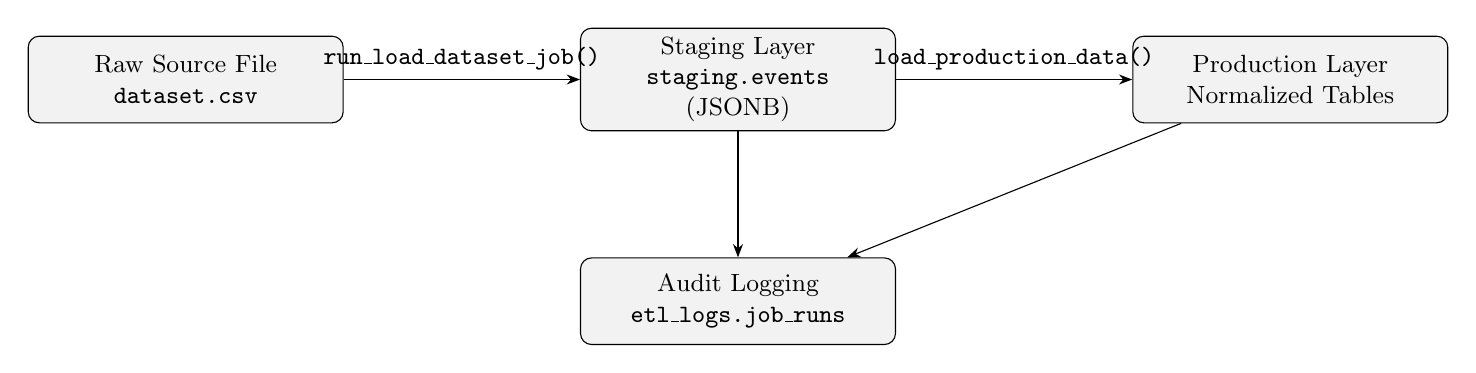
\begin{tikzpicture}[node distance=3cm, >=Stealth, font=\small]
\tikzstyle{box}=[
    draw, rounded corners,
    align=center,
    minimum width=4cm,
    minimum height=1.1cm,
    fill=gray!10
]

\node[box] (csv) {Raw Source File\\\texttt{dataset.csv}};
\node[box, right=of csv] (stg) {Staging Layer\\\texttt{staging.events}\\(JSONB)};
\node[box, right=of stg] (prod) {Production Layer\\Normalized Tables};
\node[box, below=1.6cm of stg] (log) {Audit Logging\\\texttt{etl\_logs.job\_runs}};

\draw[->] (csv) -- node[above]{\texttt{run\_load\_dataset\_job()}} (stg);
\draw[->] (stg) -- node[above]{\texttt{load\_production\_data()}} (prod);
\draw[->] (stg) -- (log);
\draw[->] (prod) -- (log);
\end{tikzpicture}
\end{center}

\captionof{figure}{Automated ETL Architecture integrating staging, normalized production, and execution logging.}
\label{fig:etl_arch}


\section{Schemas}

The database is structured in two layers to separate raw ingestion from validated, relational data storage. This supports reliability, maintainability, and independent evolution of each part of the ETL pipeline.

\subsection*{Staging Schema}

\textbf{\texttt{staging.events}}(\texttt{stagEventId SERIAL PK}, \texttt{content JSONB}, \texttt{load\_date TIMESTAMP})\\[3pt]
The staging layer acts as a \textit{landing zone} that accepts raw CSV input with minimal assumptions. All fields are ingested as JSONB to provide:

\begin{itemize}
\item \textbf{schema flexibility} when the source file evolves
\item \textbf{traceability} of original data before transformation
\item \textbf{efficient upsert checks} based on \texttt{student\_id} comparison
\item \textbf{auditable} timestamp of ingestion (\texttt{load\_date})
\end{itemize}

Only minimal uniqueness logic is applied here; validation and constraints are deferred to the production layer.

\vspace{6pt}
\subsection*{ETL Logging Schema}

\textbf{\texttt{etl\_logs.job\_runs}}(\texttt{logId PK}, \texttt{jobname}, \texttt{status}, \texttt{error\_message}, \texttt{start\_date}, \texttt{end\_date}, \texttt{records\_count})\\[3pt]
This table stores execution metadata for \texttt{pg\_cron} jobs. Helper functions such as:
\begin{center}
\texttt{return\_max\_date()}, \texttt{update\_job\_run()}, \texttt{update\_job\_skipped()}, \texttt{update\_job\_failed()}
\end{center}
standardize ETL lifecycle state transitions to \emph{running}, \emph{completed}, \emph{skipped}, or \emph{failed}.  
This provides real-world \textbf{observability} needed in automated data pipelines.

\vspace{6pt}
\subsection*{Production Schema (Normalized)}

Production tables enforce a clean, 3NF structure with strongly typed attributes. The data model is structured around the natural key \texttt{student\_id}, forming one-to-one relationships:

\begin{itemize}[leftmargin=1.4em]
  \item \textbf{\texttt{production.student}}(\texttt{student\_id PK}, \texttt{age}, \texttt{gender})\\
  \textit{Demographics:} attributes that describe a person directly.

  \item \textbf{\texttt{academic\_performance}}(\texttt{student\_id PK, FK}, GPA, SAT score, field\_of\_study)\\
  \textit{Education achievements and knowledge foundations.}

  \item \textbf{\texttt{skills\_extracurriculars}}(\texttt{student\_id PK, FK}, internships, projects, certifications, soft skills, networking score)\\
  \textit{Practical skill development and career readiness.}

  \item \textbf{\texttt{career\_outcomes}}(\texttt{student\_id PK, FK}, job offers, salary, satisfaction, promotion timeline, job level, work-life balance, entrepreneurship)\\
  \textit{Early career success indicators after graduation.}
\end{itemize}

\vspace{4pt}
To ensure relational integrity:
\begin{itemize}
\item \textbf{All foreign keys cascade on delete} — removing a student removes dependent facts.
\item \textbf{CHECK constraints} enforce valid value ranges and categorical membership.
\item \textbf{Idempotent} upserts ensure reprocessing does not create duplicates.
\end{itemize}

\vspace{3pt}
This schema structure enables efficient querying across dimensions while preserving data correctness and consistency across incremental loads.


\section{Normalization (1NF, 2NF, 3NF)}
The transformation stage restructures raw JSONB into a clean relational model that satisfies classical normalization rules. Since the dataset contains distinct thematic categories (demographics, academics, skills, career outcomes), the final schema avoids redundancy and ensures strong data integrity guarantees.

\textbf{1NF (First Normal Form).}
\begin{itemize}
\item All values in production tables are atomic and strongly typed (e.g., integers, numeric ranges, constrained enums).
\item No repeating groups or multi-valued fields are present.
\item JSONB appears only in the staging layer where schema flexibility is necessary; once validated, data moves into scalar columns.
\end{itemize}

\textbf{2NF (Second Normal Form).}
\begin{itemize}
\item Every table has a single-column primary key: \texttt{student\_id}.
\item All non-key attributes depend solely on the entire key, eliminating partial dependencies.
\end{itemize}

\textbf{3NF (Third Normal Form).}
\begin{itemize}
\item Non-key attributes do not depend on other non-key attributes.
\item Tables reflect single-subject domains: demographics, academic performance, skills development, and career outcomes are separated.
\item CHECK constraints enforce valid domains, preventing semantic anomalies.
\end{itemize}

This ensures a high-quality analytical data model: consistent updates, reduced duplication, and improved query performance.


\section{ETL Implementation Details}

The ETL pipeline operates in two independent but coordinated stages: \textbf{staging ingestion} and \textbf{production loading}. Both stages are \textbf{idempotent}, allowing safe re-execution without creating duplicate or inconsistent data.

\subsection*{Staging Loader (Change-Aware Upsert)}

\textbf{Function:} \texttt{run\_load\_dataset\_job()}\\[4pt]
This function implements \textbf{incremental ingestion} by detecting whether the source CSV has changed:

\begin{enumerate}[leftmargin=1.6em]
\item Check file modification timestamp using:\newline
\texttt{pg\_stat\_file('/app/dataset.csv').modification}
\item Compare with \texttt{MAX(end\_date)} from previous successful executions of job \textit{dataset-load}.
\item If the file is updated or first ingestion occurs:
    \begin{itemize}
      \item Bulk-load into a temporary table via \texttt{COPY}
      \item Convert each row to JSONB
      \item \textbf{UPDATE} existing rows only if content changed
      \item \textbf{INSERT} new rows if \texttt{student\_id} not present
    \end{itemize}
\item If no change is detected, the job status is set to \texttt{skipped} to avoid redundant writes.
\end{enumerate}

\textbf{Benefits:}
\begin{itemize}
\item Reduced I/O load (\textbf{only changed data is written})
\item Safe repeated execution without corrupting data
\item Full traceability because raw data stays in staging
\end{itemize}

Execution status, error messages, and the number of affected records are automatically written to the audit table \texttt{etl\_logs.job\_runs}, which improves debugging and operational monitoring in a real production environment.

\subsection*{Production Loader (Idempotent Upsert)}

\textbf{Function:} \texttt{load\_production\_data()}\\[4pt]
This function transforms validated data from \texttt{staging.events} into a fully normalized production schema. JSONB fields are cast into strongly typed columns, while \texttt{INSERT \ldots ON CONFLICT DO UPDATE} ensures that loading is \textbf{idempotent}: data can be refreshed repeatedly without creating duplicates or losing referential integrity.

\textbf{Processing Steps}:
\begin{enumerate}[leftmargin=1.6em]
\item Extract typed values from JSONB using
      \verb|content->>'field'|
\item \textbf{Insert or update} into:
    \begin{itemize}
      \item \texttt{production.student} — demographics
      \item \texttt{production.academic\_performance} — education metrics
      \item \texttt{production.skills\_extracurriculars} — practical skill indicators
      \item \texttt{production.career\_outcomes} — workforce success measures
    \end{itemize}
\item Domain rules are applied automatically through:
    \begin{itemize}
      \item \textbf{CHECK constraints} (e.g., GPA/score ranges)
      \item \textbf{foreign key enforcement} with cascading deletes
    \end{itemize}
\end{enumerate}

\textbf{Benefits}:
\begin{itemize}
\item Guarantees synchronized data between staging and production
\item Maintains consistency even under repeated execution or partial failures
\item Enforces relational correctness before acceptance into the analytical layer
\end{itemize}

This stage completes the ETL pipeline by transforming semi-structured raw input into reliable, query-optimized relational data.

\section{Automation (Scheduling with \texttt{pg\_cron})}

The entire pipeline is automated using the PostgreSQL extension \texttt{pg\_cron}, enabling scheduled SQL tasks to run inside the database without external tools.

\textbf{Configuration:}
\begin{itemize}
\item Extension installed in Docker image: \texttt{postgresql-16-cron}
\item PostgreSQL configuration updated:
\begin{verbatim}
shared_preload_libraries = 'pg_cron'
cron.database_name = 'test_db'
\end{verbatim}
\item Scheduler becomes active as soon as the container initializes
\end{itemize}

\textbf{Recurring Jobs Deployed in This Project:}
\begin{itemize}[leftmargin=1.4em]
  \item \texttt{load-dataset} job — runs \textbf{every 1 minute} \\
        \texttt{SELECT run\_load\_dataset\_job();}
        \begin{itemize}
            \item detects changes in the source file
            \item ingests and upserts raw data into staging
        \end{itemize}

  \item \texttt{etl-job} — runs \textbf{every 2 minutes} \\
        \texttt{SELECT load\_production\_data();}
        \begin{itemize}
            \item normalizes staged data into production tables
            \item enforces integrity and validation rules
        \end{itemize}
\end{itemize}

Both tasks are created automatically during initialization using:
\begin{center}
\texttt{SELECT cron.schedule(\ldots);}
\end{center}

\textbf{Operational Impact:}
\begin{itemize}
\item Data freshness is continuously preserved
\item Historical job runs are fully auditable via \texttt{etl\_logs.job\_runs}
\item No human intervention required after deployment
\end{itemize}

Thus, the system behaves like a real production ETL pipeline, combining automation, monitoring, and resilience in a fully containerized environment.

\section{Deployment \& Reproducibility}

A major requirement of this project was to ensure a fully automated and reproducible deployment process. To achieve this, the entire ETL stack (PostgreSQL 16, pg\_cron scheduler, staging + production schemas, and jobs) is packaged inside a Docker image. Upon container startup, the entire system self-configures, eliminating any need for manual SQL execution.

\subsection*{Docker Image and Initialization}

\textbf{Dockerfile Highlights:}
\begin{itemize}[leftmargin=1.4em]
  \item Based on the official \texttt{postgres:16} image, ensuring reliability and security.
  \item Installs the \textbf{pg\_cron} extension, activating in-database automation.
  \item Configures:
  \begin{verbatim}
  shared_preload_libraries = 'pg_cron'
  cron.database_name = 'test_db'
  \end{verbatim}
  \item Automatically copies initialization SQL scripts and the dataset:
        \begin{itemize}
        \item schema creation (staging, production, logging)
        \item ETL functions (\texttt{run\_load\_dataset\_job()}, \texttt{load\_production\_data()})
        \item pg\_cron job scheduling
        \end{itemize}
  \item Zero manual configuration is required — the pipeline becomes operational at first boot.
\end{itemize}

This setup ensures consistency across environments and supports rapid redeployment in case of failures.


\subsection*{Build \& Run Instructions}

Running the ETL system locally or on any server requires just two terminal commands:

\begin{enumerate}[leftmargin=1.5em]
  \item \textbf{Build the image:}
        \begin{verbatim}
        docker build -t dbd-pipeline .
        \end{verbatim}
  \item \textbf{Start a container:}
        \begin{verbatim}
        docker run --name dbd-pg -p 5432:5432 \
            -e POSTGRES_PASSWORD=postgres dbd-pipeline
        \end{verbatim}
\end{enumerate}

Once launched, PostgreSQL automatically:
\begin{itemize}
\item creates schemas and tables,
\item loads and normalizes data,
\item registers two scheduled ETL jobs with pg\_cron,
\item begins continuous ingestion and transformation.
\end{itemize}

Users can immediately connect with:
\begin{verbatim}
psql -h localhost -U postgres -d test_db
\end{verbatim}

\textit{Reproducibility is guaranteed}: the same results are produced regardless of the machine running the container, fulfilling modern DevOps and data engineering deployment standards.

\section{Logging \& Monitoring}
\texttt{etl\_logs.job\_runs} captures: job name, status, timestamps, error message, and processed record counts. Helper functions consistently transition statuses from \emph{running} to terminal states. Use:
\begin{lstlisting}[language=SQL]
SELECT * FROM etl_logs.job_runs ORDER BY logId DESC LIMIT 20;
\end{lstlisting}

\section{Analysis: Issues \& Improvements (Requirement \#7)}

The implemented solution successfully demonstrates a fully automated ETL pipeline, but also reveals several practical challenges and opportunities for enhancement.

\subsection*{Strengths and Successful Design Choices}
\begin{itemize}[leftmargin=1.4em]
  \item \textbf{Idempotent ETL:} UPSERT logic ensures that data synchronization remains correct even under repeated executions or system restarts.
  \item \textbf{Change-aware ingestion:} Incremental loading based on file modification timestamps minimizes I/O and avoids unnecessary churn in the staging layer.
  \item \textbf{Strict normalization:} Moving from JSONB to strongly typed 3NF tables reduces redundancy, isolates update responsibilities, and improves query quality.
  \item \textbf{Full automation:} The pipeline operates continuously without human intervention, automatically triggering staging and production loads at scheduled intervals.
  \item \textbf{Operational observability:} Detailed run metadata (status, timestamps, error causes, row counts) enables reliable monitoring and debugging.
\end{itemize}

\subsection*{Identified Limitations}
\begin{itemize}[leftmargin=1.4em]
  \item \textbf{Dataset coupling to container:} Since \texttt{dataset.csv} is bundled into the Docker image, updating data requires a full rebuild instead of hot reloading.
  \item \textbf{Staging schema has minimal validation:} Malformed or missing fields in the input may only be detected later during production load.
  \item \textbf{Split ETL stages may cause temporary inconsistency:} If staging succeeds but production fails, data may be in a partially refreshed state until the next scheduled run.
  \item \textbf{Performance scalability:} JSONB queries and full-table scans may become costly as dataset size grows beyond a few thousand records.
\end{itemize}

\subsection*{Planned Improvements}
\begin{itemize}[leftmargin=1.4em]
  \item \textbf{External dataset volume + checksum-based change detection:} Mounting the input file via Docker volume and checking SHA256 fingerprints would enable dynamic updates and stronger change validation.
  \item \textbf{Transactional production load:} Wrapping the full \texttt{load\_production\_data()} execution inside a single transaction ensures all-or-nothing consistency.
  \item \textbf{Early validation rules in staging:} Introducing JSON schema or \texttt{CHECK} constraints (e.g., numeric casting) at ingestion time would reduce rejected rows during later processing.
  \item \textbf{Indexing strategy:} Adding dedicated indexes on \texttt{(content->>'student\_id')} and foreign-key columns improves lookup performance during upserts.
  \item \textbf{Extended monitoring:} Tracking execution duration and error categories would provide more actionable operational insights in production environments.
\end{itemize}

\subsection*{Overall Assessment}
The current system fully satisfies project requirements by integrating automation, normalization, and incremental data refresh. The listed improvements would further enhance maintainability, fault tolerance, and scalability, making the pipeline suitable for real-world workloads with continuously evolving datasets.


\section*{Appendix A: File Map}
\begin{longtable}{>{\ttfamily}p{0.36\linewidth}p{0.56\linewidth}}
\toprule
01\_database\_setup.sql & Create DB, schemas (\texttt{staging, production, etl\_logs}), enable extensions.\\
02\_staging\_schema.sql & Staging table, job log table, staging loader \& helper functions, cron job for ingestion.\\
03\_production\_schema.sql & Production tables with constraints, production loader function, cron job for ETL.\\
Dockerfile & PostgreSQL 16 + pg\_cron; copies dataset and init scripts; sets preload libraries.\\
install.sh & Convenience script to install Docker and Compose on Ubuntu.\\
\bottomrule
\end{longtable}

\section*{Compilation Notes}
This document uses standard \LaTeX{} packages. Compile with \texttt{latexmk -pdf DBD\_Documentation.tex}. If you see a ``rerun'' notice, compile a second time to refresh bookmarks/outlines.

\end{document}
